
\documentclass[a4paper,12p]{article}

% used to specify page dimentions
\usepackage[includeheadfoot,margin=2.5cm]{geometry}

% used to modify the header and the footer
\usepackage{fancyhdr}
\pagestyle{plain}

% used to change font (for this to work you need to change your engine to xelatex or luatex)
\usepackage{fontspec}
\setmainfont{Times New Roman}

% used to change paragraph spacing and line spacing
\usepackage{setspace}
\centering
\setlength{\parskip}{6pt}
\renewcommand{\baselinestretch}{1.5}

% used to set default section and subsection font sizes and spacing and style
\usepackage{titlesec}
\usepackage{sectsty}

\titleformat*{\section}{\fontsize{14pt}{12pt}\bfseries\raggedright}
\titleformat*{\subsection}{\fontsize{12pt}{6pt}\bfseries\raggedright}
\titleformat*{\subsubsection}{\fontsize{10pt}{5pt}\bfseries\raggedright}

% used to set the numbering of sections and subsections and subsubsection
\renewcommand\thesection{\arabic{section}}
\renewcommand\thesubsection{\thesection.\arabic{subsection}}
\renewcommand\thesubsubsection{}

% used to generate random text, use \lipsum[n] where n is the number of paragraphs
\usepackage{lipsum}

% for lists
\usepackage{enumitem}
\setlist{nosep}

% for images
\usepackage{graphicx}
\userpackage{float}
\graphicspath{{images/}}
\usepackage[figurename=Figure]{caption}
\renewcommand{\figurename}{Figure}

\begin{document}
    % write content here
    % you will get a compilation error if this section is empty

    % add title

    % add authors
     \begin{center}
        \textbf{Raid Nasrellah TEYAR} \\
        \textbf{Oussama SALAHOUELHADJ} \\
        \textbf{Mohammed Elhadi SAOUDI} \\
    \end{center}

     \raggedright\section{Les besion fonctionnelle}

    
     \subsection{Actor: Teacher responsible of the module}
        \subsubsection{Authentication functional requirements:}
        \begin{itemize}
            \item Login.
            \item reset password.
        \end{itemize}

        \subsubsection{Modul management functional requirements:}
        \begin{itemize}
            \item Consult his own modules.
        \end{itemize}

        \subsubsection{Question bank/module management functional requirements:}
        \begin{itemize}
            \item Consult the bank of questions.
        \end{itemize}

        \subsubsection{Question management functional requirements:}
        \begin{itemize}
            \item Create a question.
            \item Modify a question.
            \item Delete a question.
            \item Consult a question.
        \end{itemize}

        \subsubsection{Exam management functional requirements:}
        \begin{itemize}
            \item Create an exam.
            \item Modify an exam.
            \item Delete an exam.
            \item Consult an exam.
            \item Try an exam.
            \item Confirm the evaluation of an exam's responses.
            \item Consult exam analytics.
            \item Assign an exam to an exam session.
            \item Export an exam.
        \end{itemize}

        \subsubsection{Response management functional requirements:}
        \begin{itemize}
            \item Consult the list of response.
            \item Consult a response.
            \item Evaluate a response.
        \end{itemize}

        \subsubsection{Claims management functional requirements:}
        \begin{itemize}
            \item Consult the list of claims.
            \item Consult a claim.
            \item Mark claim as solved.
            \item Report student.
            \item Reply to a claim.
            \item Modify a reply.
        \end{itemize}

        \item Modify his own profile.


     \subsection{Actor: Teacher responsible of the td/tp}
     \subsubsection{Authentication functional requirements:}
     \begin{itemize}
         \item Login.
         \item reset password.
     \end{itemize}

     \subsubsection{Question bank management functional requirements:}
     \begin{itemize}
         \item Consult the bank of questions.
     \end{itemize}

     \subsubsection{Question management functional requirements:}
     \begin{itemize}
         \item Create a question.
         \item Modify a question.
         \item Delete a question.
         \item Consult a question.
     \end{itemize}

     \subsubsection{Exam management functional requirements:}
     \begin{itemize}
         \item Consult exam analytics.
     \end{itemize}

     \subsubsection{Response management functional requirements:}
     \begin{itemize}
         \item Consult list of responses.
         \item Consult a response.
         \item Evaluate a response.
     \end{itemize}

     \item Modify his own profile.

     \subsection{Actor: Student}
     \subsubsection{Authentication functional requirements:}
     \begin{itemize}
         \item Login.
         \item reset password.
     \end{itemize}

     \subsubsection{Exams schedule management functional requirements:}
     \begin{itemize}
         \item Consult list of exams.
         \item Consult an exam.
         \item Set a reminder for an exam.
     \end{itemize}

     \subsubsection{Pass an exam functional requirements:}
     \begin{itemize}
         \item Test requirements.
         \item Check in for exam.
         \subsubsection{Communicate with the proctor of an exam:}
         \begin{itemize}
             \item rise hand to talk to a proctor.
             \item write a message to a proctor.
             \item consult messages from a proctor.
         \end{itemize}

         \item give feedback about an exam.
         \item leave an exam.
         \item consult results of exam.
     \end{itemize}

     \subsubsection{Claims functional requirements:}
     \begin{itemize}
        \item Claim an evaluation of a question.
        \item Consult a claim.
     \end{itemize}

     \subsubsection{Absence functional requirements:}
     \begin{itemize}
         \item Justify an absence.
         \item Consult a response.
     \end{itemize}

     \item Modify his own profile


     \subsection{Actor: Admin}
     \subsubsection{Authentication functional requirements:}
     \begin{itemize}
         \item Login.
         \item reset password.
     \end{itemize}

     \subsubsection{User management functional requirements:}
     \begin{itemize}

        \subsubsection{Teacher management functional requirements:}
         \begin{itemize}
             \item Consult list of teachers.
             \item add a teacher.
             \item modify teacher.
             \item delete a teacher.
             \item consult a teacher.
             \item affect modules to a teacher.
         \end{itemize}

         \subsubsection{Student management functional requirements.}
         \begin{itemize}
             \item consult list of students.
             \item add a student.
             \item modify a student.
             \item delete a student.
             \item consult a student.
         \end{itemize}

     \end{itemize}

     \subsubsection{Module management functional requirements:}
     \begin{itemize}
        \item consult list of modules.
        \item add a module.
        \item modify a module.
        \item delete a module.
        \item consult a module.
     \end{itemize}

     \subsubsection{Exam management functional requirements:}
     \begin{itemize}
        \item Create an exam session.
        \item modify an exam session.
        \item Delete an exam session.
        \subsubsection{Exam's proctors management:}
         \begin{itemize}
            \item Assign a proctor to an exam.
            \item Consult list of proctors.
            \item Modify proctor.
            \item Dismiss a proctor from an exam.
         \end{itemize}
         \item Consult analytics of an exam.
         \item Notify students.
         \subsubsection{Absence justification management:}
         \begin{itemize}
            \item consult list of absence justifications.
            \item consult an absence justification.
            \item mark an absence justification as done.
            \item replay to an absence justification.
            \item modify replay.
         \end{itemize}
     \end{itemize}

     \subsubsection{Report management functional requirements:}
     \begin{itemize}
         \item consult list of reports.
         \item consult a report.
         \item mark a report as done.
         \item replay to a report.
     \end{itemize}

     \item Backup configuration and database.
     \item Restore configuration and database.
     \item Modify his own profile.

     \subsection{Actor: Proctor}
     \subsubsection{Authentication functional requirements:}
     \begin{itemize}
         \item Login.
         \item reset password.
     \end{itemize}

     \subsubsection{Exam session management functional requirements:}
     \begin{itemize}
        \subsubsection{Control session:}
         \begin{itemize}
             \item start a session.
             \item End exam session.
             \item Enable exit exam for students.
             \item Disable exit exam for students.
             \item Enable enter exam for student.
             \item Disable enter exam for students.
             \item Confirm presence list.
         \end{itemize}
         \subsubsection{Communicate with student:}
         \begin{itemize}
             \item Speak to all students.
             \item Speak to a student.
             \item Message all students.
             \item Message a student.
            \end{itemize}
            \subsubsection{Session proctoring functional requirements:}
            \begin{itemize}
                \item Proctor students.
                \item Pin a student
                \subsubsection{Proctoring a student:}
                \begin{itemize}
                    \item proctor a student.
                    \item write a comment about a student.
                    \item End session for a particular student.
             \end{itemize}
         \end{itemize}
        \item Consult exam analytics.
     \end{itemize}
    
     \item Modify his own profile.

     \section{Diagrame global }
     \begin{figure}[h]
         \centering
         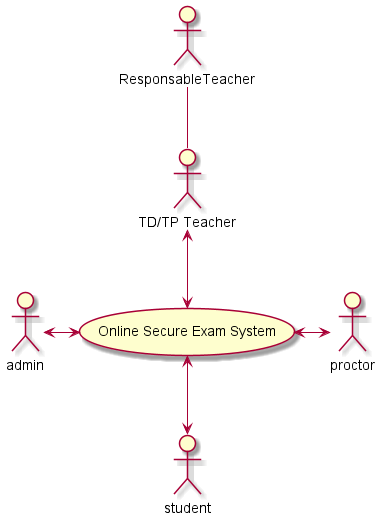
\includegraphics[width=200pt]{SCD}
         \caption{static global diagram}
     \end{figure}
     \clearpage
     \section{DCU de chaque acteur}
     \vspace{5cm} %5mm vertical space
     % when using images you just have to include the name of the image without the extension

    \begin{figure}[h]
        \centering
        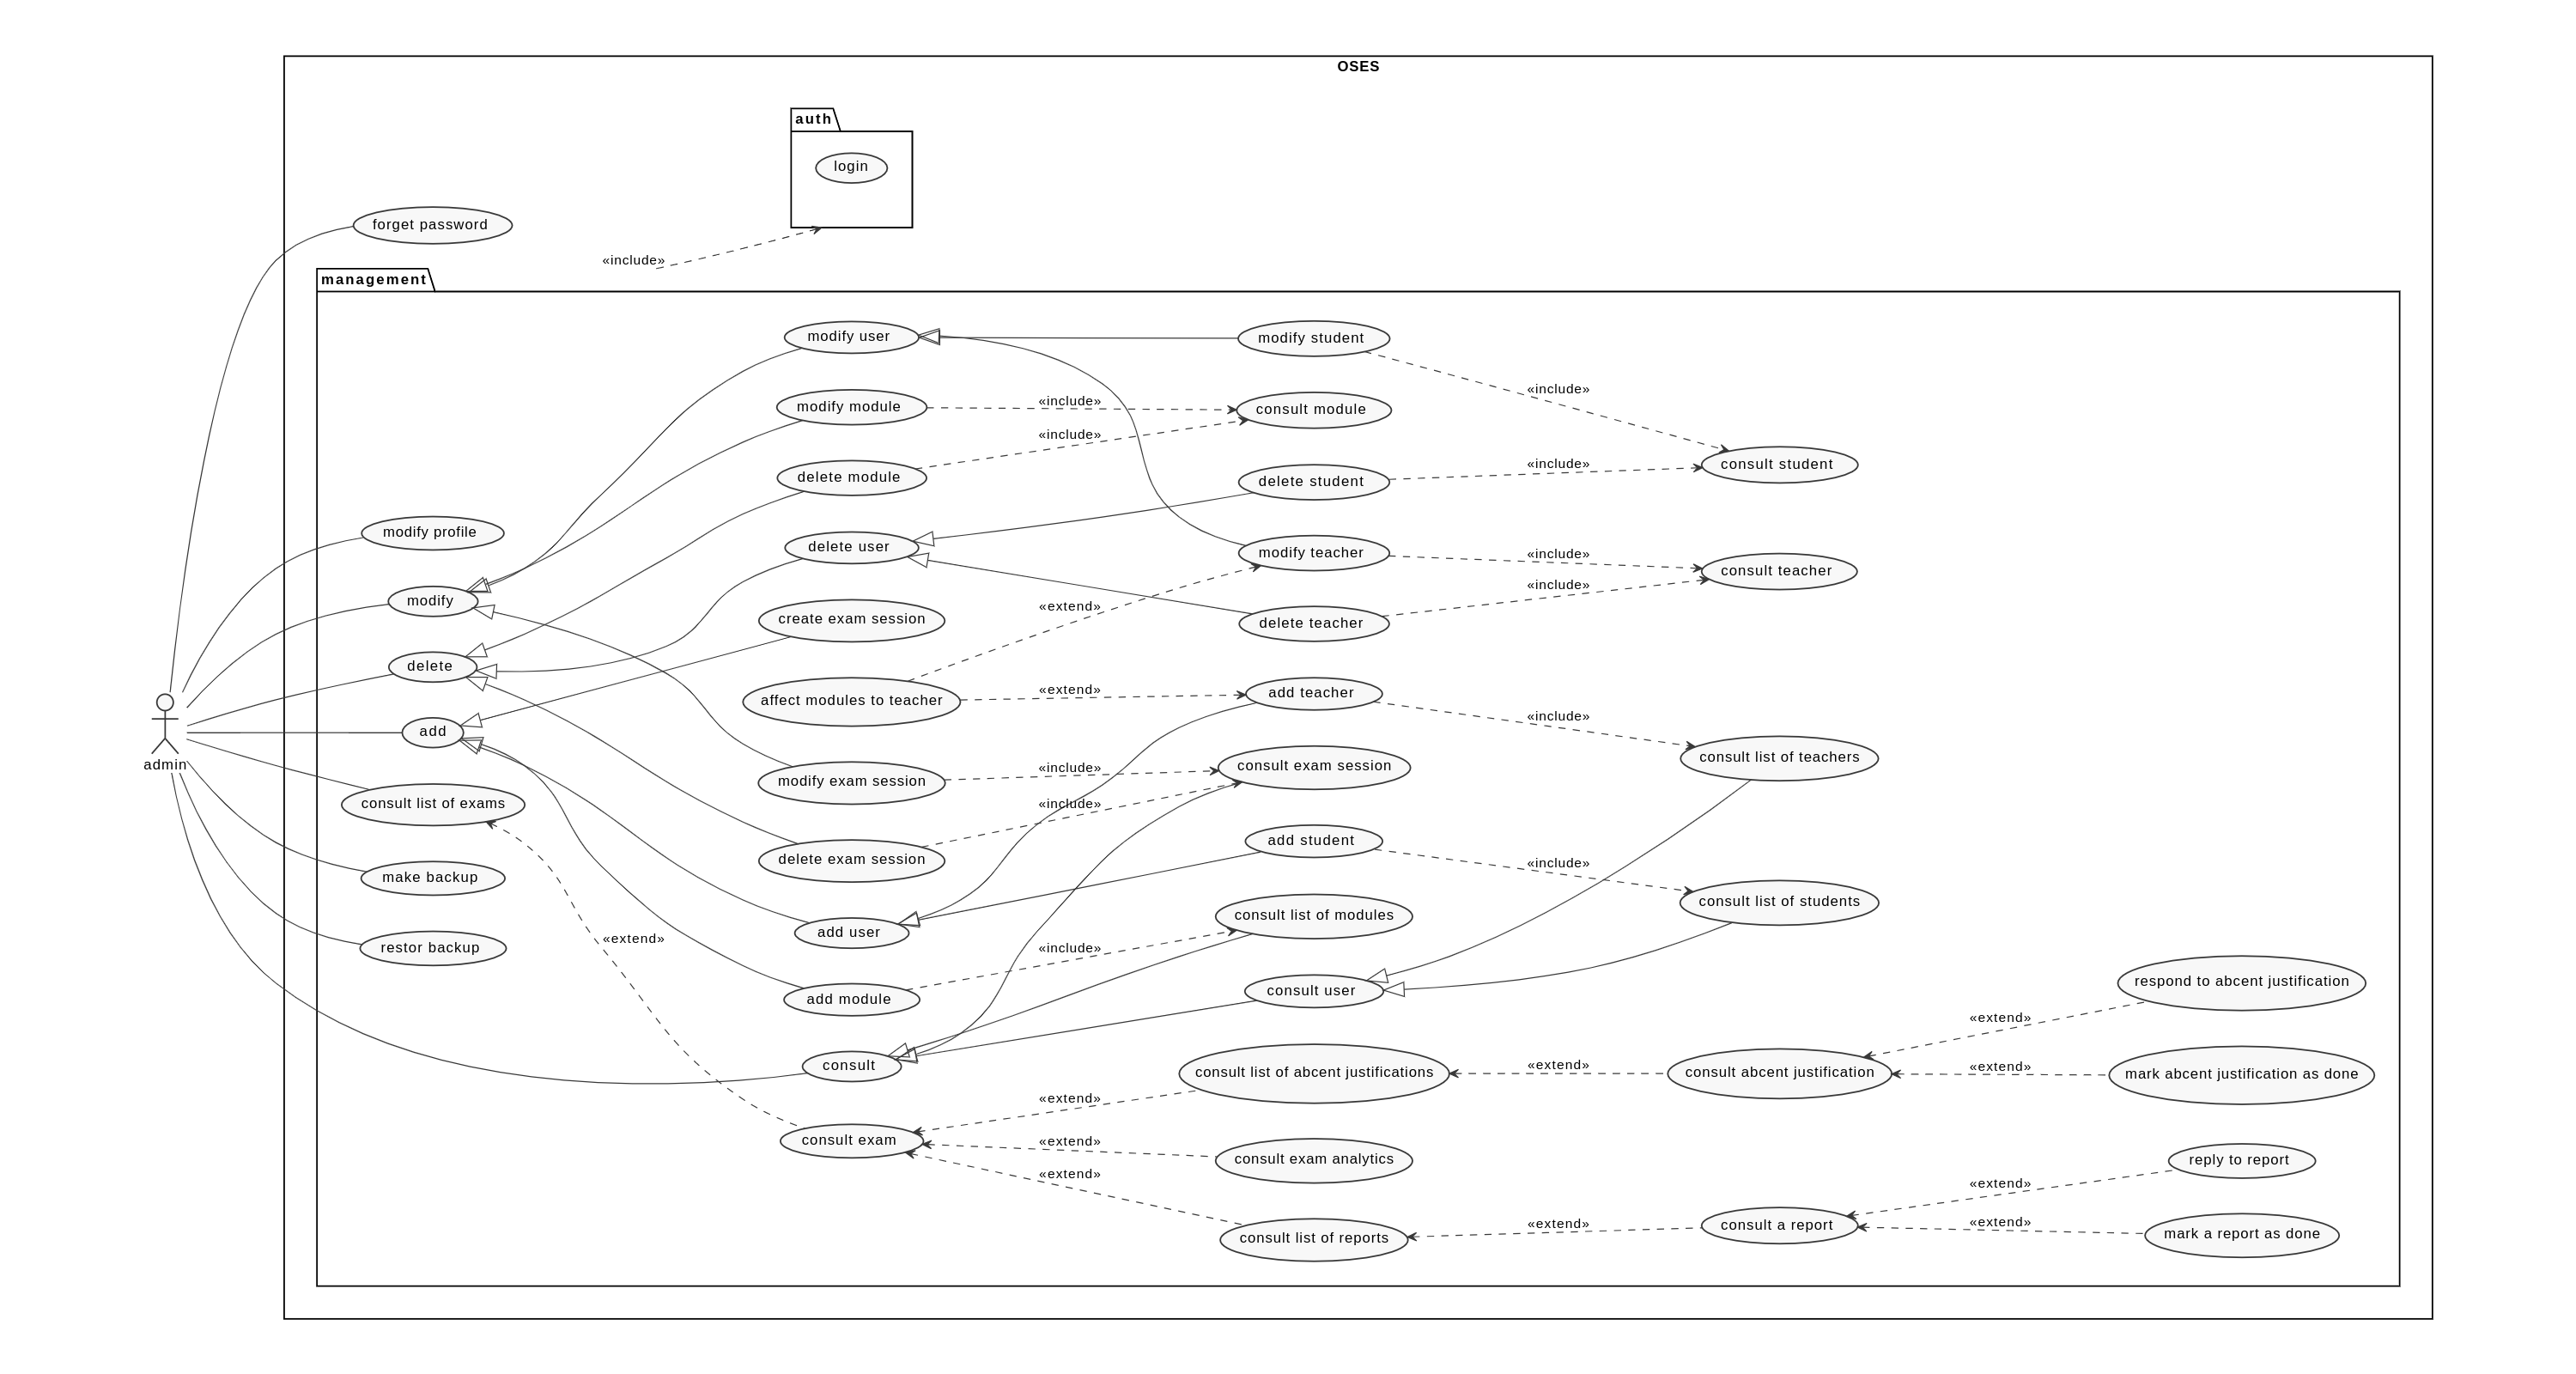
\includegraphics[width=\textwidth]{admin_UCD}
        \caption{admin use case diagram}
    \end{figure}

     \begin{figure}[h]
         \centering
         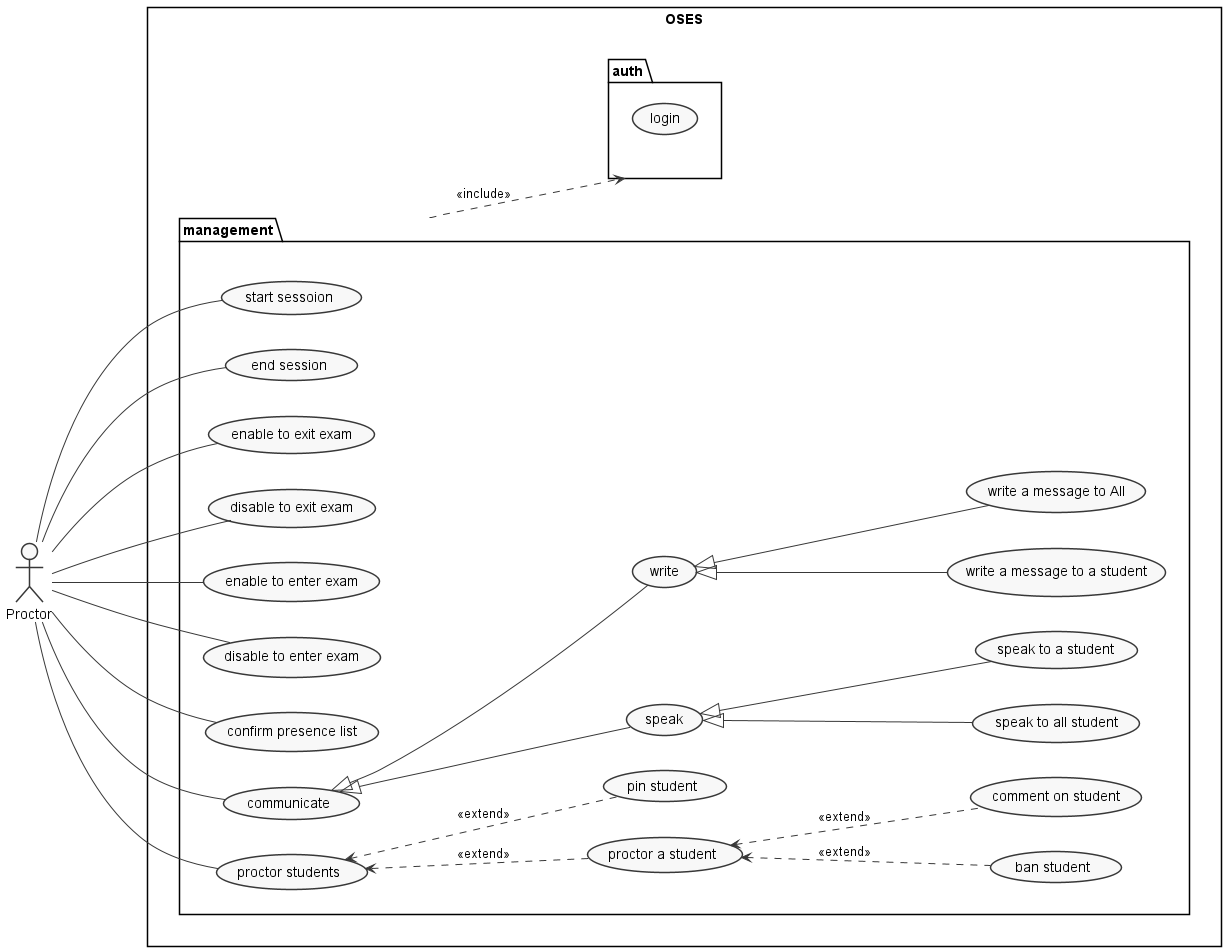
\includegraphics[width=\textwidth]{proctor_UCD}
         \caption{proctor use case diagram}
     \end{figure}

    \begin{figure}[h]
        \centering
        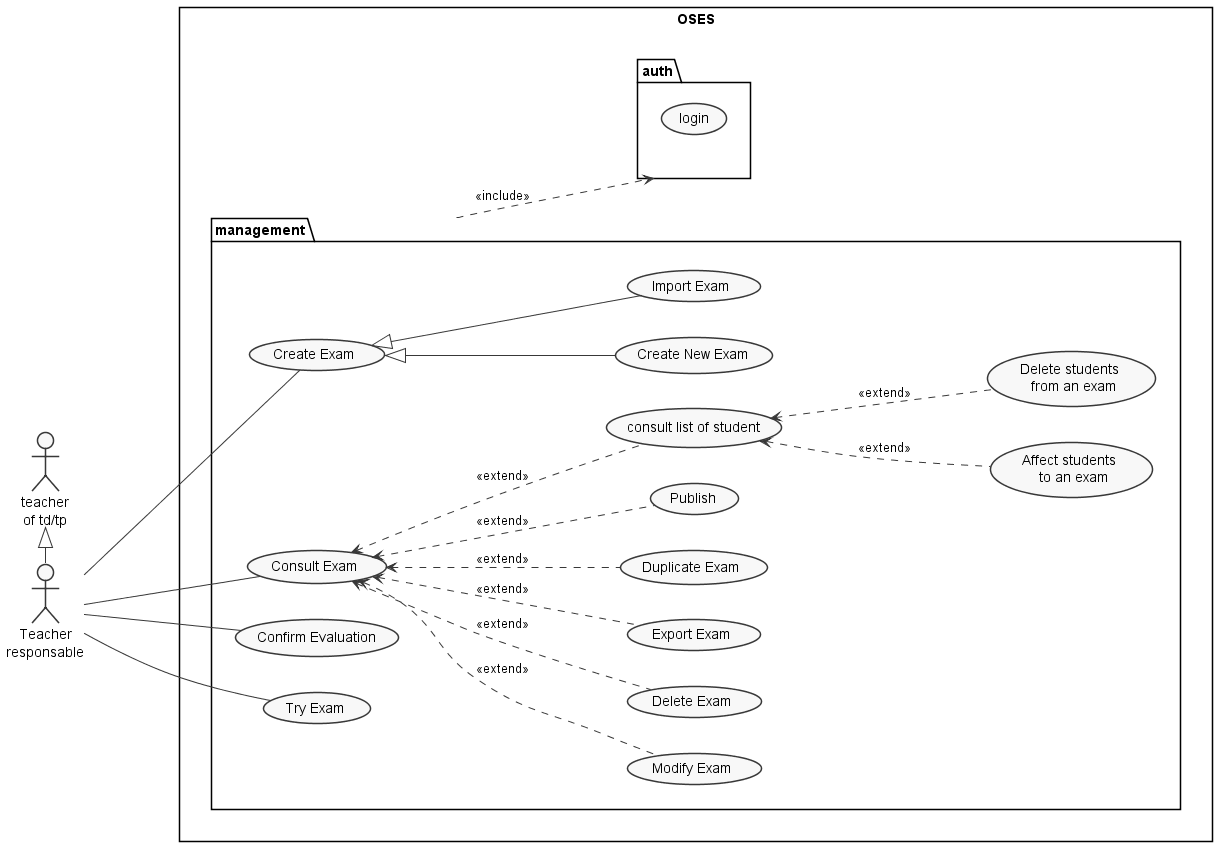
\includegraphics[width=450pt]{Module_Teacher}
        \caption{module teacher use case diagram}
    \end{figure}

    \begin{figure}[h]
        \centering
        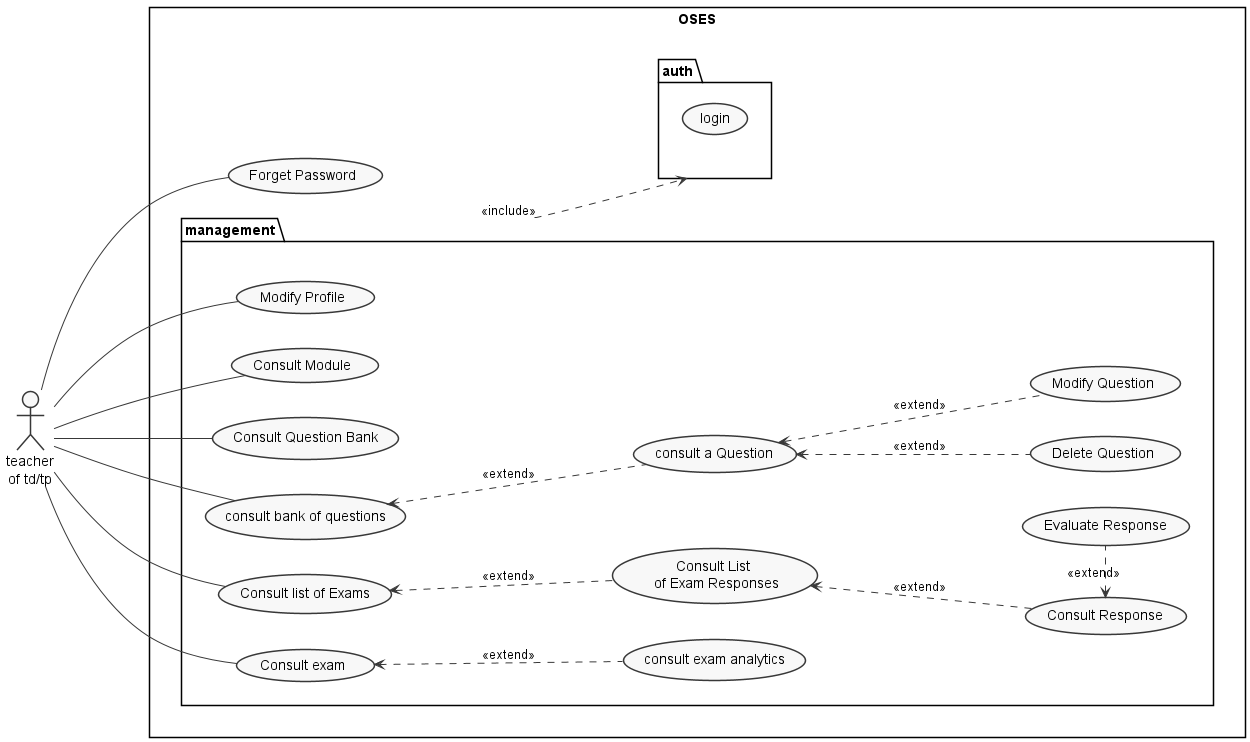
\includegraphics[width=\textwidth]{TP_TD_Teacher}
        \caption{Td/Tp teacher use case diagram}
    \end{figure}

    \begin{figure}[h]
        \centering
        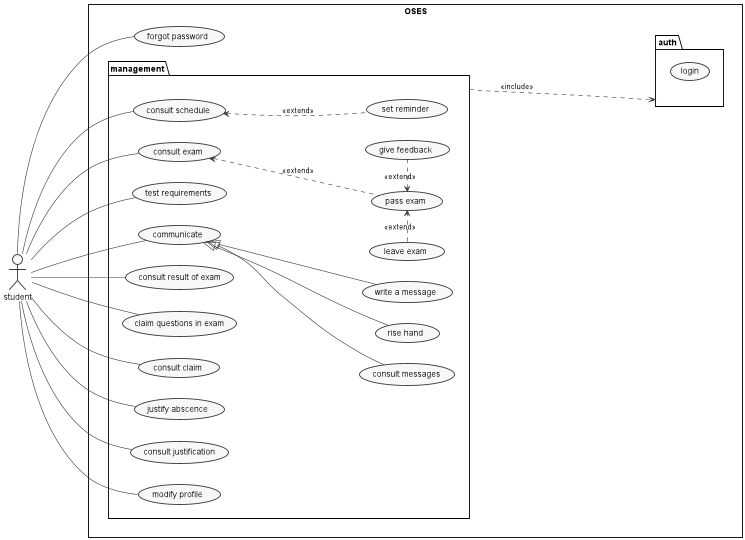
\includegraphics[width=350pt]{student_UCD}
        \caption{student use case diagram}
    \end{figure}


\end{document}